\section{System Overview}
\label{sec-system-overview} 
We implemented a holistic system for shoulder surfing, with the neural network as core, on a smartphone to verify the efficiency of our model. It iterates through the following steps: 

\vspace{1mm}
\noindent
\textbf{Input:} Under the guidance of the attacker, The smartphone will zoom in, take focus, and take several images(the number is freely adjustable) with burst mode of the target screen. As digital zooming does not put in any extra data, we'll only use maximum optical zooming(if exist) when photographing to reduce the workload of neural networks.

\vspace{1mm}
\noindent
\textbf{Alignment:} The images are then aligned to mitigate tremors. Luckily, in our scenario the target is a glowing screen whose edges are easily distinguishable in most cases, and we use them as reference to align our images. The images are also spun to make the text horizontal in the process. The screen is cropped out and the rest of the image abandoned.


\vspace{1mm}
\noindent
\textbf{Adjustment:} The lines of text(or stuff differing from the background color of the screen) will be carved out for processing to reduce the workload of the network. The character size is normally 10 to 20 pixels, while variations in size aren't influential as they're covered in the training data, so zooming isn't necessary.

\vspace{1mm}
\noindent
\textbf{Processing:} As our SR network accepts only 9$\times$9 patches, we will process all the 9$\times$9 patches (with overlapping) among the input photo to generate 36$\times$36 images (4$\times$ upscaling). The input is RGB colored, while the output, as we are not interested in color, is black and white. The three calculation processes (Alignment, Adjustment, Processing) run parallel to the input process so that the attacker can process a batch of images while the next batch is being collected simultaneously.
		
\vspace{1mm}
\noindent
\textbf{Output:} The outputs of our SR network, the 36$\times$36 overlapping patches, are then rearranged to their original locations and merged (using average values) into a single image. As we only carve out the texts for processing, we will then insert these high-res texts back to their original locations on one of the input images, and display the patched image to the attacker (An illustration of the patched image can be found in Fig.~\ref{illustration_of_system}).

These steps are repeatedly executed to enable the attacker to monitor the victim at an interval of 1 to 2 seconds. At critical times requiring continuous monitoring so as not to miss transient display, e.g. password entering, the system can simply lengthen the input phase across that period and process the data afterwards. The workflow of our system is shown in Figure~\ref{fig-workflow}.
\begin{figure}
  \centering
     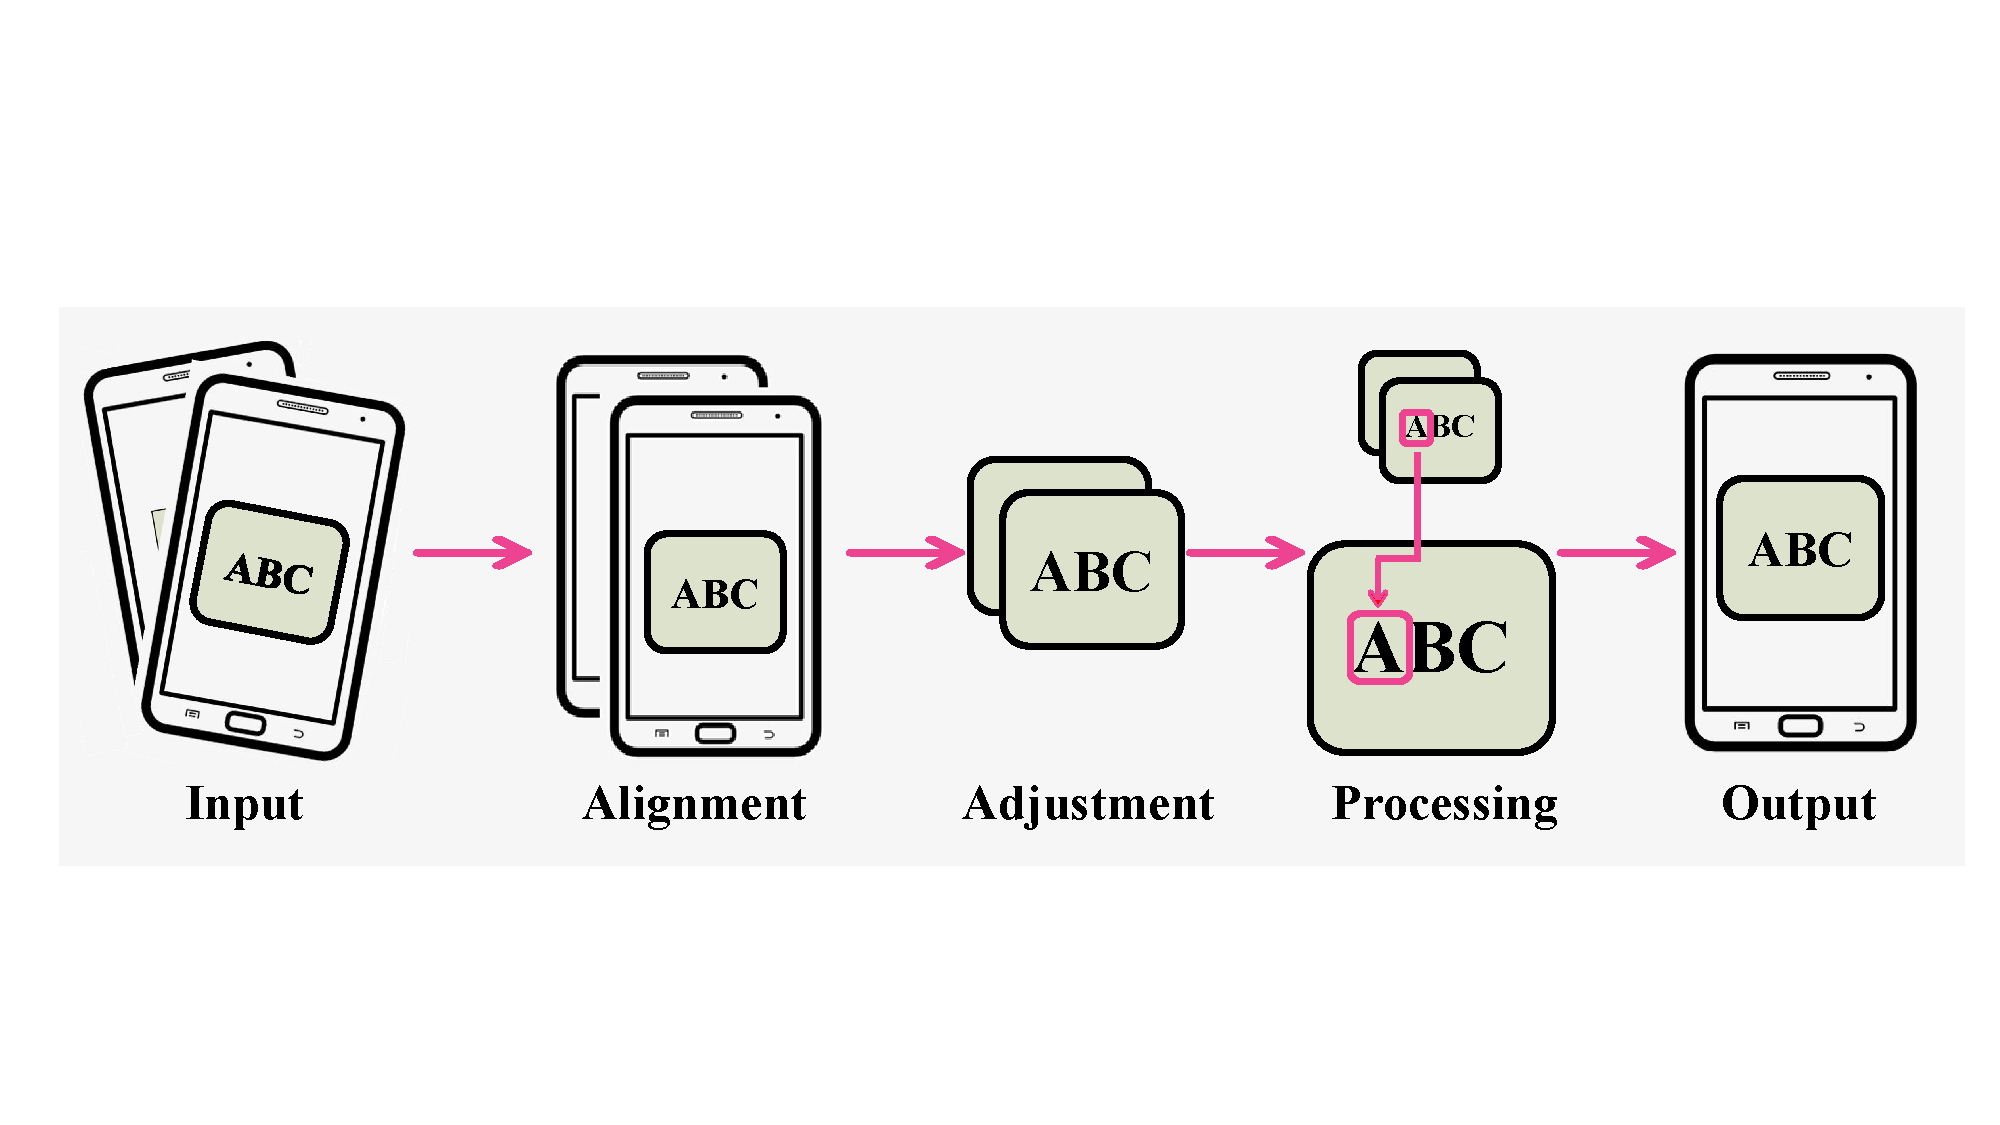
\includegraphics[width=0.90\linewidth]{./pic/workflow_cl.pdf}
     \caption{Workflow of the \textsf{SRPeek} system.}
     \label{fig-workflow}
\end{figure}


